\documentclass{article}

\author{Tran Van Tan Khoi}

\title{Weekly Homework Report \#3}

\date{April 7, 2025}

\usepackage[T1]{fontenc}
\usepackage[utf8]{inputenc}
\usepackage[a4paper,top=2cm,bottom=2cm,left=3cm,right=3cm,marginparwidth=1.75cm]{geometry}
\usepackage[colorlinks=true, allcolors=blue]{hyperref}
\usepackage{bookmark}
\usepackage{graphicx}
\usepackage{dirtree}


\begin{document}

\maketitle

\section{Introduction}
\label{introduction}

In this report, I attempt to demonstrate how sorting algorithms' running time compare when organizing integers data in ascending order. I will show how I achieved in getting the results using only C++ source files and libraries. At the same time, I attempt to give a deep dive into different categories of sorting algorithms, how each algorithm performs in certain cases, and their possible applications. Stay tuned as I show you, a race to show who is the fastest in replacing and reorder positive values in a particular order for convenient use in the future.

All of the files of this project, including this report, is available at \href{https://github.com/xtrkoi/throwaway-rep}{my Github repository}.


\section{Overview}
\label{overview}

This experiment covers basic key aspects, including C++ implementations of sorting algorithms; a way to generate different types of data that needs to be reorganize; a way to measure the running time and all the number of comparisons; and a way to compile the results into a table of data, for the convenience of drawing charts so we can compare and judge the competitors. However, this experiment is lacking in a proper benchmark library (e.g. \href{https://github.com/google/benchmark}{Google's Benchmark Library}) and a generic implementation that support any comparable data type and any compare function. With that being said, the results should still give a good demonstration of how these algorithms perform in the real world.


\subsection{Structure}
\label{stucture}

This project includes numerous folders and files, organized as follow:

\begin{itemize}
	\item \textbf{bin}: This folder contains the binary files, \texttt{datagen.exe}, \texttt{main.exe}, and \texttt{sorter.exe}. The purpose of each binary file is explained later with their respective C++ source file counterpart.
	\item \textbf{data}: This folder contains various \texttt{.txt} files and a \texttt{benchmark.csv} file that contain intermediary sorting data and all running time results.
	\item \textbf{docs}: This folder contains various files for a \LaTeX \space project that compiles this very report you are reading, which beside discussing the resulting running times and number of comparisons of sorting algorithms, also explaining how this project works, how you can import your own sorting data and experiment with each algorithm implemented here.
	\item \textbf{libs}: This folder includes the header files for the sorting algorithms and methods of generating data for testing.
	\item \textbf{logs}: This folder includes the logs of running programs.
	\item \textbf{util}: This folder includes source files for supporting running the project.
	\item \texttt{main.cpp}: The main source file that will execute the majority actions of the project.
\end{itemize}


\pagebreak

\begin{figure}
	% \centering
	\dirtree{%
		.1 root.
		.2 bin.
		.3 datagen.exe.
		.3 main.exe.
		.3 sorter.exe.
		.2 data.
		.3 benchmark.csv.
		.3 tmp.
		.3 input.txt.
		.3 answer.txt.
		.3 <name>.txt.
		.2 docs.
		.3 report.tex.
		.3 report.pdf.
		.2 libs.
		.3 include.
		.3 src.
		.3 tests.
		.2 logs.
		.2 util.
		.3 datagen.cpp.
		.3 sorter.cpp.
		.2 main.cpp.
	}
	\caption{The folder structure}
\end{figure}

\subsection{Tests}
\label{tests}

This experiment is performed on Windows 11 operating system on Performance mode, build 23H2, running on Intel's Core Ultra 7 155H (4.8 GHz/24 MB), 16 GB LPDDR5X RAM, and 1TB M.2 NVMe PCIe 4.0 SSD. Please consult the table below.

\vrule

\begin{tabular}{c|c}
	% \caption{Benchmark Specifications}
	Processor        & Intel Core\texttrademark \space Ultra 7 155H (4.8 GHz Boost, 24 MB Cache) \\
	Memory           & 16 GB 7467 MT/s LPDDR5X                                                   \\
	Storage          & 1 TB NVMe PCIe 4.0                                                        \\
	Operating System & Windows 11 Build 23H2, Performance Mode                                   \\
	Compiler         & GNU G++23
\end{tabular}

\subsection{Usage}
\label{usage}

\subsubsection*{sorter.cpp}

Build the source file with the following command (at root folder):

\begin{verbatim}
    g++ .\util\sorter.cpp .\libs\src\*.cpp -o .\bin\sorter -O2
\end{verbatim}


And run with

\begin{verbatim}
    .\bin\sorter
\end{verbatim}


Optional flags:

\begin{itemize}
	\item \textbf{-a}: Choosing which algorithm to run. C++ \texttt{std::sort} is run by default.
	\item \textbf{-i}: Direct input stream from file given by path.
	\item \textbf{-o}: Direct output stream to file given by path.
\end{itemize}


\subsubsection{datagen.cpp}

Build the soruce file with the following command (at root folder):

\begin{verbatim}
    g++ .\util\datagen.cpp .\libs\tests\*.cpp -o .\bin\datagen -O2
\end{verbatim}


And run with

\begin{verbatim}
    .\bin\datagen
\end{verbatim}


Optional flags:

\begin{itemize}
	\item \textbf{-s}: The size of the data to be generated (at most $5\cdot10^6$)
	\item \textbf{-t}: The type of data to be generated (\texttt{random}, \texttt{sorted}, \texttt{reversed}, \texttt{nearly}, or \texttt{repeated});
	\item \textbf{-o}: Direct the output stream to file given by path.
\end{itemize}


\subsubsection*{main.cpp}

Build the soruce file with the following command (at root folder):

\begin{verbatim}
    g++ main.cpp .\libs\src\*.cpp .\libs\tests\*.cpp  -o .\bin\main -O2
\end{verbatim}


And run with

\begin{verbatim}
    .\bin\main
\end{verbatim}

which will run all sorting algorithms with all data types and sizes, storing each resulting run in \texttt{data/benchmark.csv}.

\subsection{Storing Data}

The input data and the sorted output of each algorithm is stored in the \texttt{data} folder.


\section{Algorithms}

\begin{enumerate}
	\item Bubble Sort
	\item Shaker Sort
	\item Selection Sort
	\item Insertion Sort
	\item Heap Sort
	\item Merge Sort (recursive and iterative variant)
	\item Quick Sort
	\item Standard Sort (\texttt{std::sort} from C++ STL)
	\item Radix Sort
	\item Counting Sort
	\item Shell Sort
	\item Flash Sort
\end{enumerate}


\pagebreak


\section{Results}


\subsection{Random Data}


\begin{figure*}[ht]
	\centering
	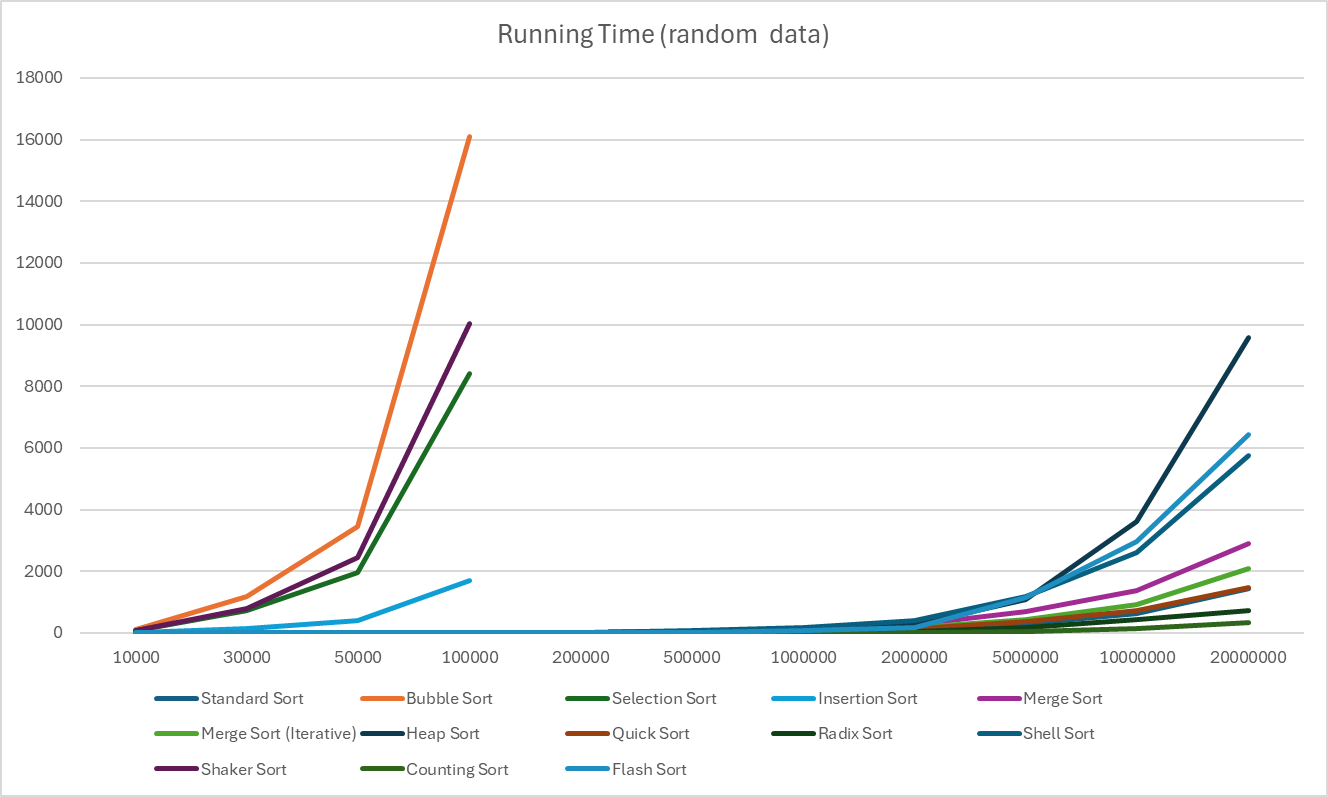
\includegraphics[width=14cm]{images/time_random.png}
\end{figure*}

\begin{figure*}[ht]
	\centering
	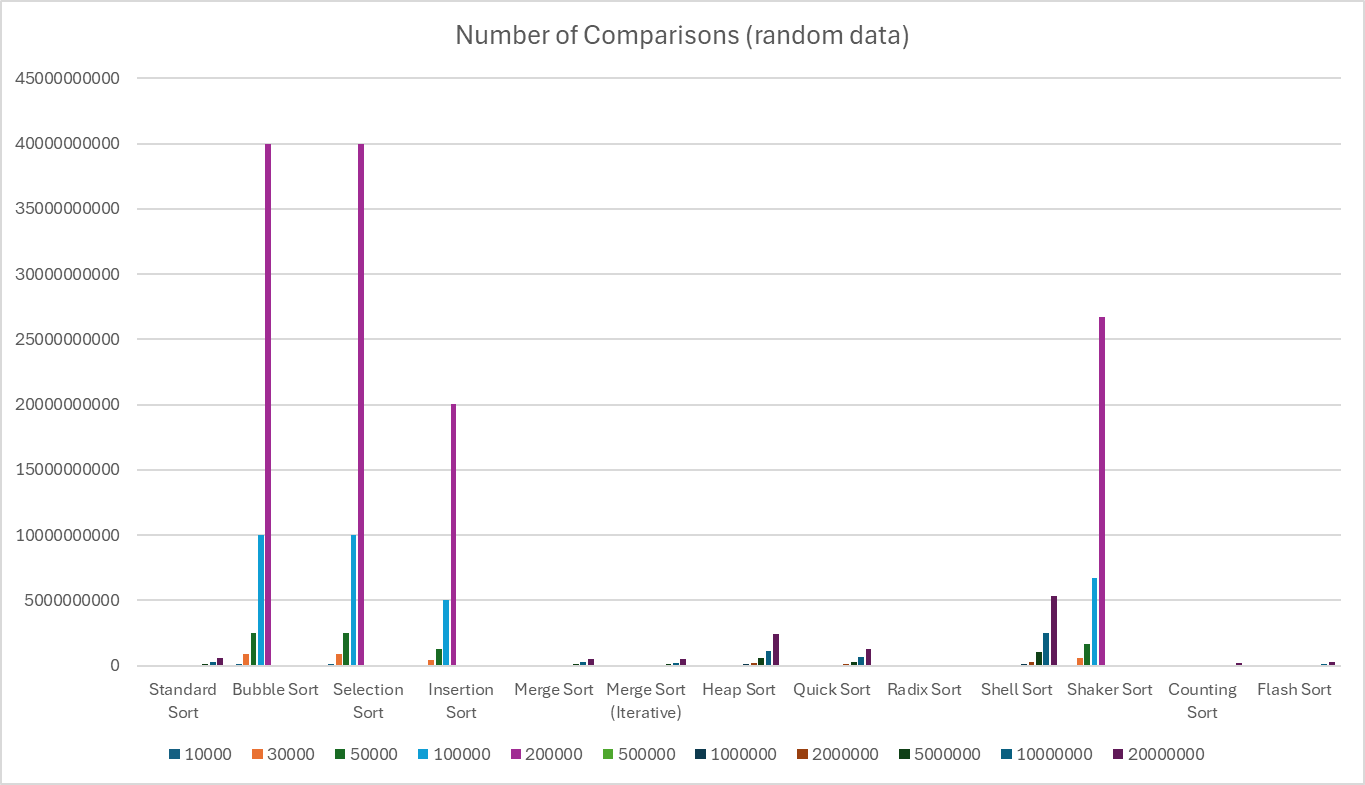
\includegraphics[width=14cm]{images/comp_random.png}
\end{figure*}


\pagebreak


\subsection{Sorted Data}

\begin{figure*}[ht]
	\centering
	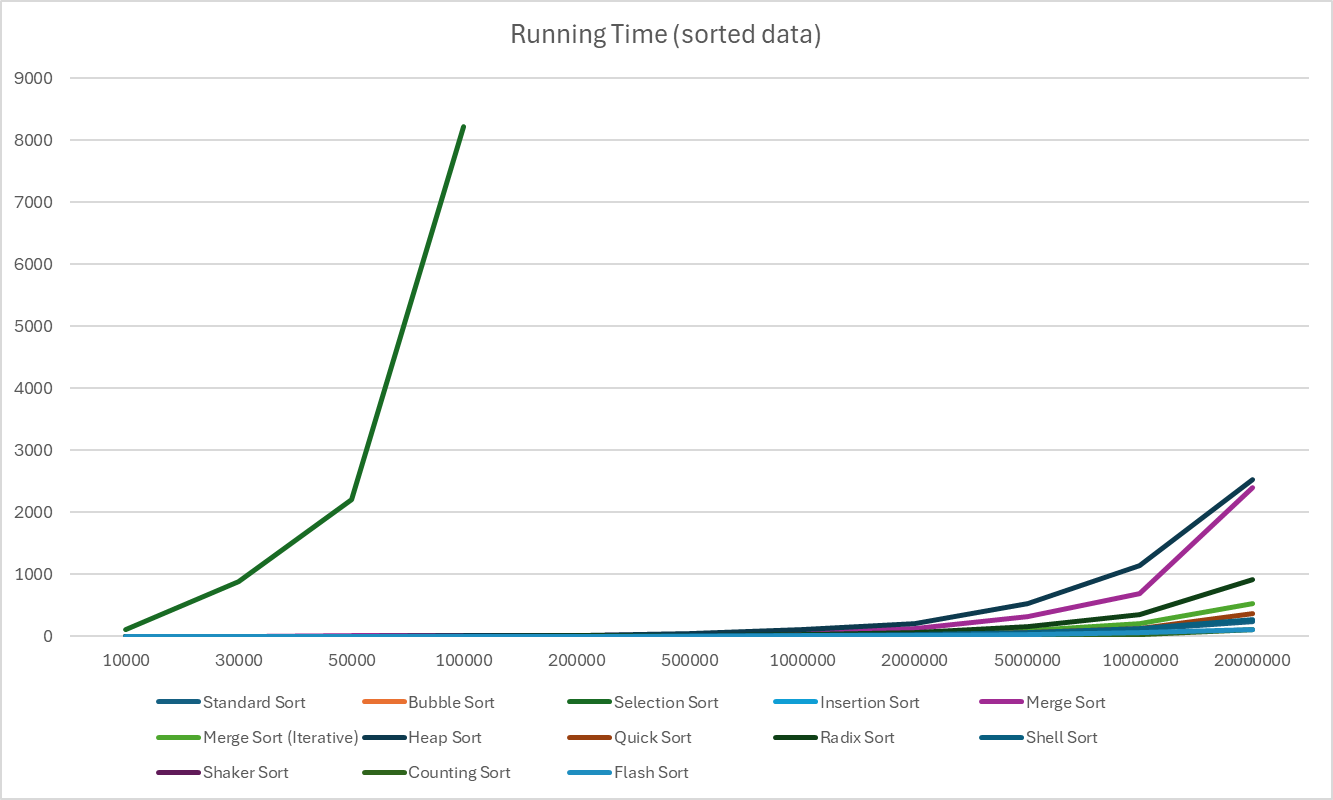
\includegraphics[width=14cm]{images/time_sorted.png}
\end{figure*}

\begin{figure*}[ht]
	\centering
	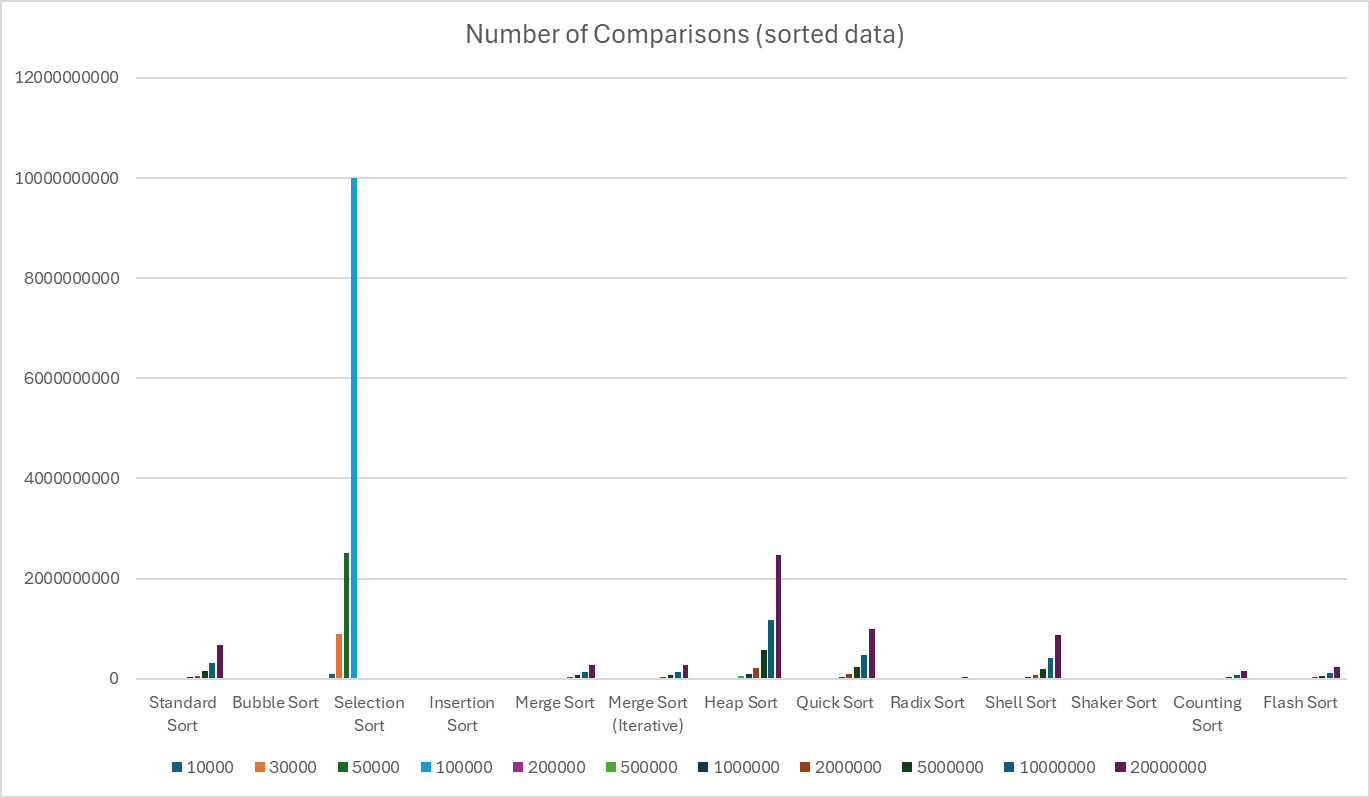
\includegraphics[width=14cm]{images/comp_sorted.png}
\end{figure*}


\pagebreak


\subsection{Reversed Sorted Data}

\begin{figure*}[ht]
	\centering
	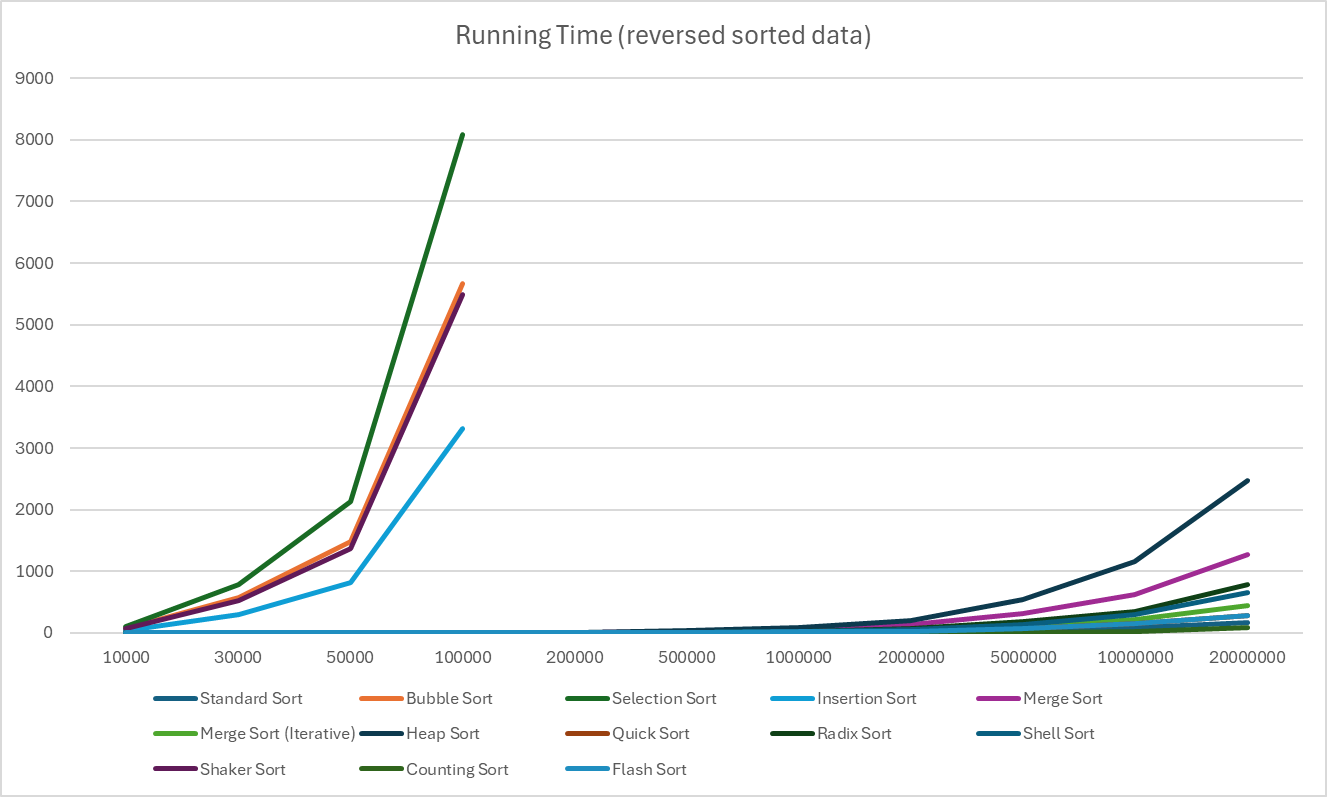
\includegraphics[width=14cm]{images/time_reversed.png}
\end{figure*}

\begin{figure*}[ht]
	\centering
	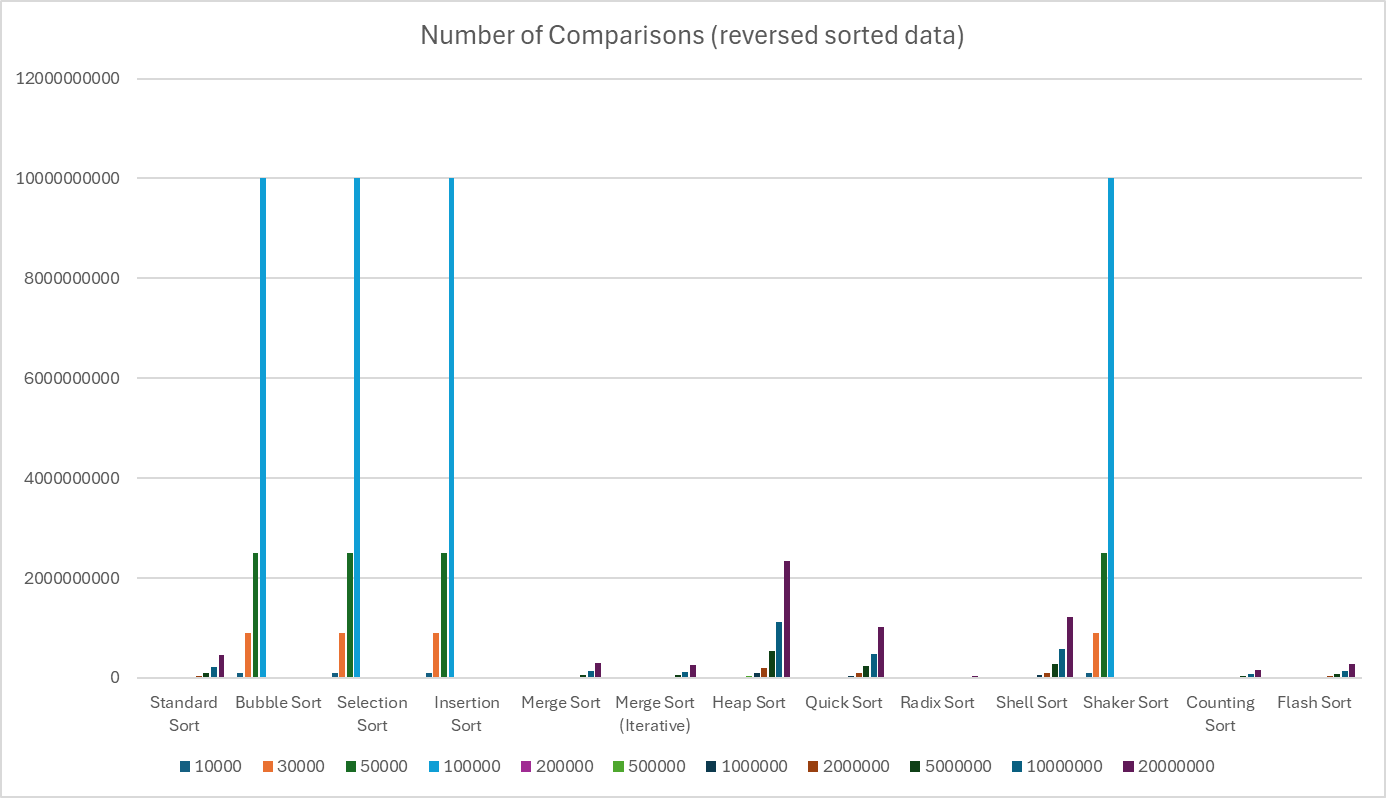
\includegraphics[width=14cm]{images/comp_reversed.png}
\end{figure*}


\pagebreak


\subsection{Nearly Sorted Data}

\begin{figure*}[ht]
	\centering
	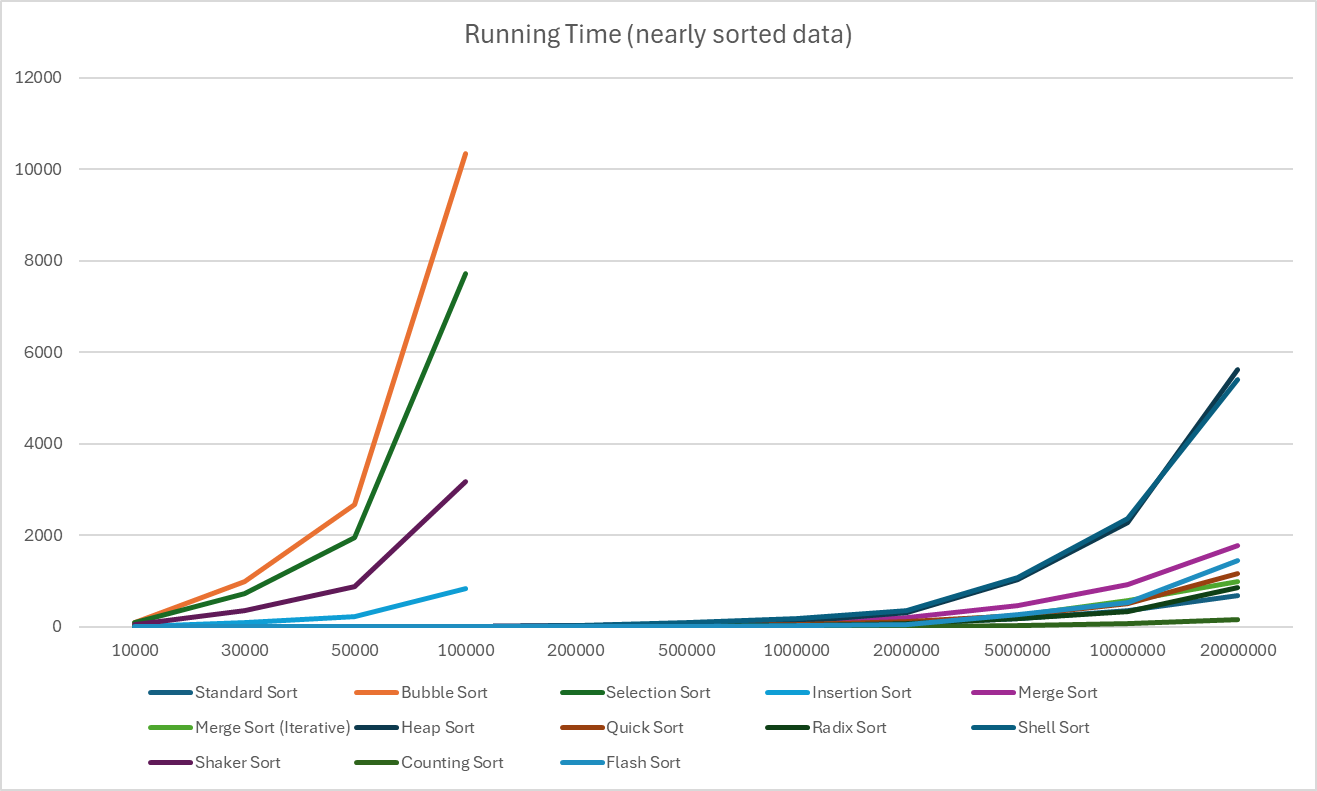
\includegraphics[width=14cm]{images/time_nearly.png}
\end{figure*}

\begin{figure*}[ht]
	\centering
	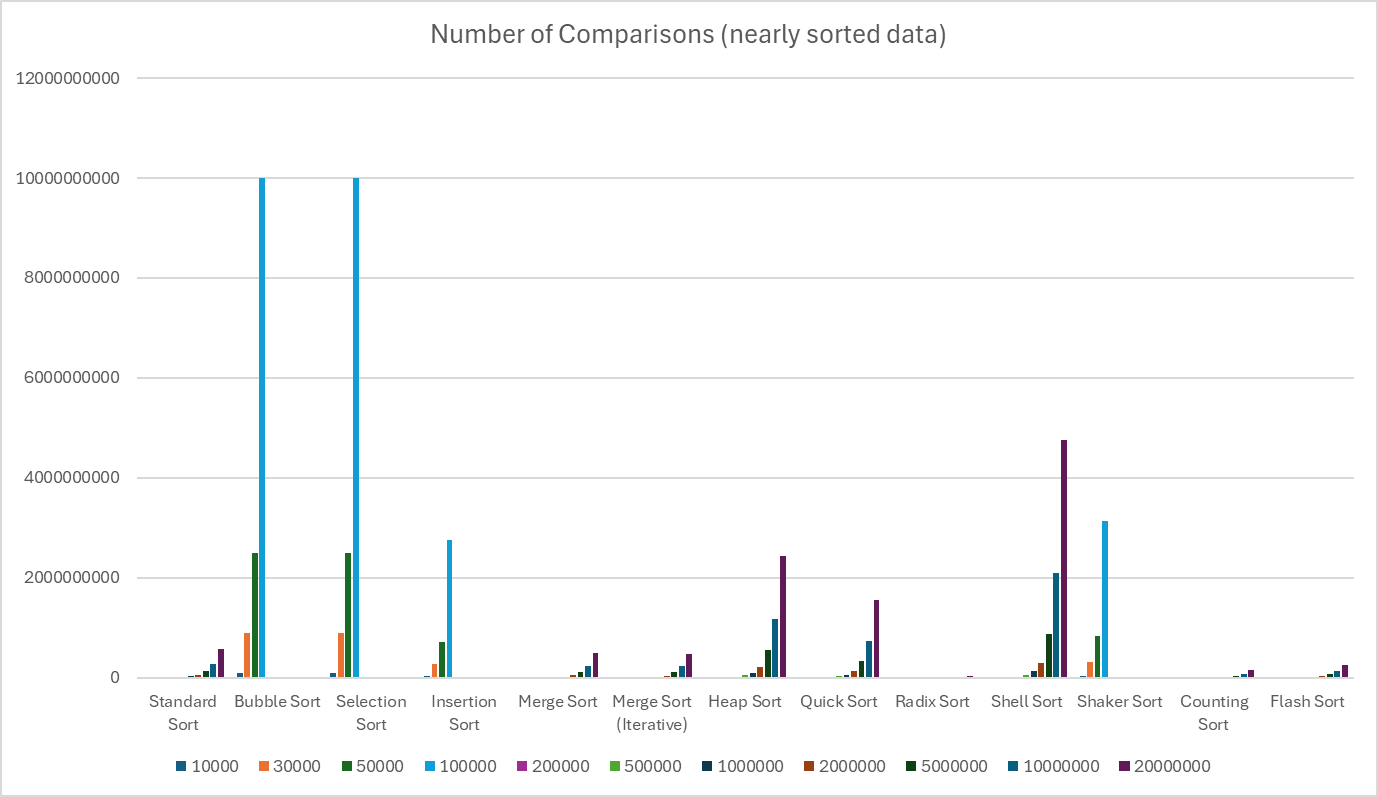
\includegraphics[width=14cm]{images/comp_nearly.png}
\end{figure*}


\pagebreak


\subsection{Data with Many Duplicates}

\begin{figure*}[ht]
	\centering
	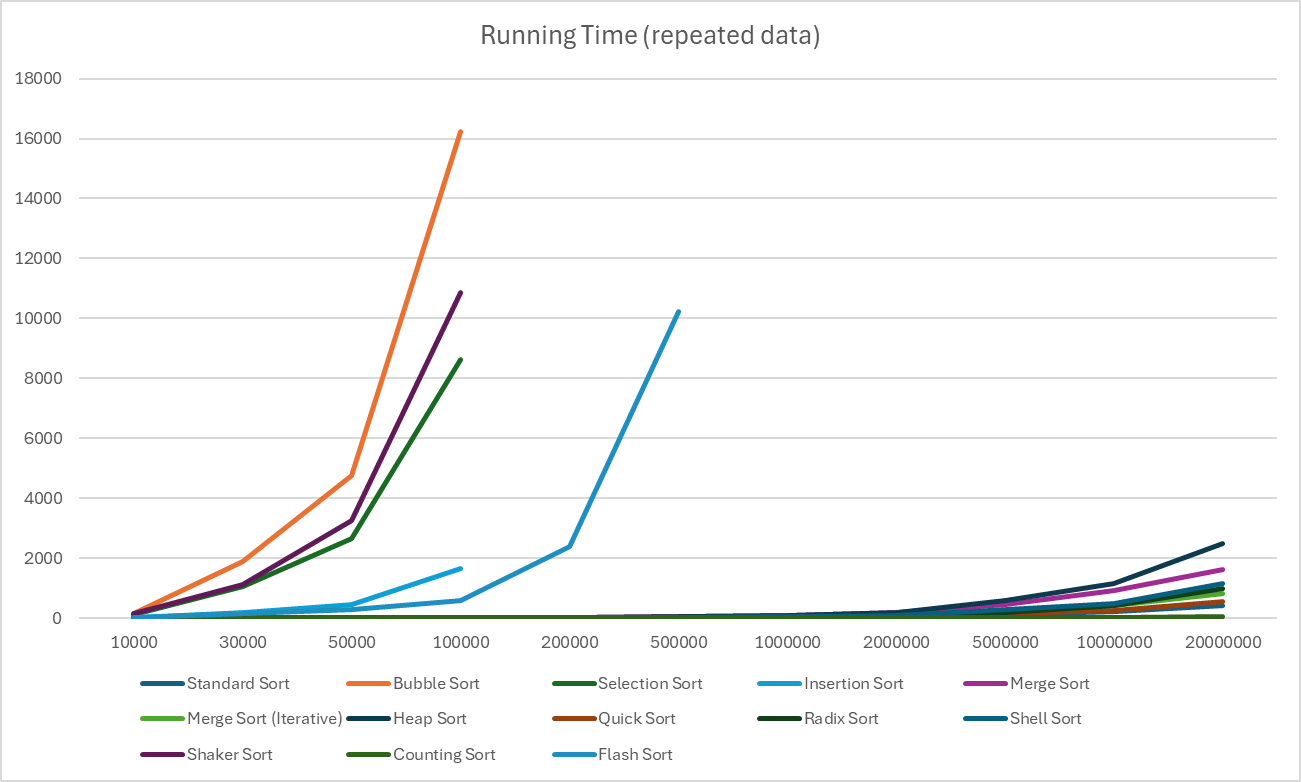
\includegraphics[width=14cm]{images/time_repeated.png}
\end{figure*}

\begin{figure*}[ht]
	\centering
	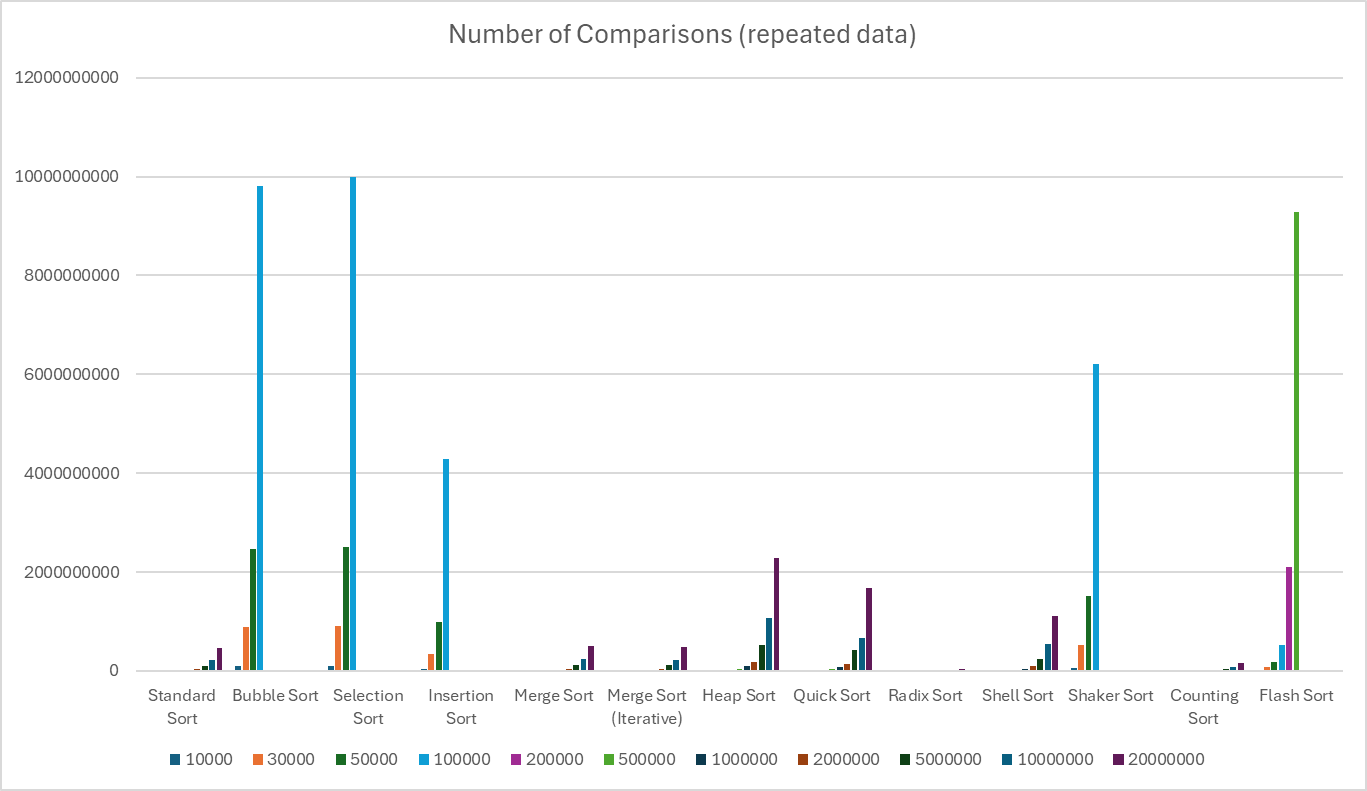
\includegraphics[width=14cm]{images/comp_repeated.png}
\end{figure*}


\pagebreak


\section{Conclusion}

This experiment demonstrated how different sorting algorithms perform in many typical scenarios in terms of running time and number of comparisons made. The quadratic solutions are simple, easy to implement and run fast for small data with little to no overhead. However, they start to fall behind when the data is significantly large. This is where faster algorithms are used instead. Quasilineaer algorithms are compatible with any types of data and act as "general-purpose sorting tool" but have some drawbacks such as overhead in recursion calls or extra memory. Linear algorithms typically run the fastest, but they usually only work with certain type of data.

However, this experiment failed to demonstrate other aspect of sorting data, such as comparable data types other than \texttt{int}, and memory footprint in certain environments.

\end{document}